\section{Password Authentication}
\label{section:password-authentication}

Passwords are one of the most common and oldest forms of user authentication, being first used in computers at MIT in the mid-60s \cite{mcmillan2012password}.

We need to understand the high-level model of password authentication, its risks and tools to mitigate it.

\subsubsection{Authentication Model}

Password authentication is a simple model based on a shared secret between the user and the system. The secret is usually a set of characters or words memorised by the user, inputted via a keyboard. We refer to it as the password.
We often used the password in a combination with a username.
To authenticate, the user simply needs to prove to the system his knowledge of the password.


\begin{figure}[h]
	\centering
	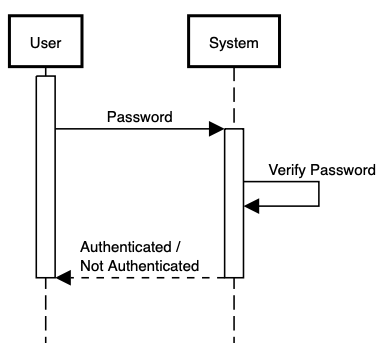
\includegraphics[height=8cm]{images/password-authentication}
	\caption{Password Authentication Model}
	\label{fig:password-authentication}
\end{figure}

\subsection{Security Vulnerabilities}
\label{label:password-vulnerabilities}

In a common password authentication system used on the web, the user sends a plain-text password over a secure HTTPS connection, the server verifies it and responds.
The simplicity that makes passwords practical for users makes them a vulnerability for systems that rely on them.

Authors \cite{conklin2004password} have shown that users pick passwords that are easier to remember and reuse the same passwords across different websites.
Many websites also don't properly handle passwords, enabling attackers to access plain-text passwords when a security breach happens.
These vulnerabilities that can result in mild inconveniences to serious offences like identity theft.
The industry is aiming to improve password security with the adoption of password managers and initiatives like FIDO \cite{cho2014passwordless} working to retire passwords altogether.

The National Institute of Standards and Technology \cite{grassi2017} classifies attacks as \textit{online} or \textit{offline}, based on how the attacker is interacting with the system.

%Security measures against online attacks can be implemented independently, regardless of the underlying authentication system, while offline attacks exploit data directly used by the authentication system.
%For this reason preventive measures need to be accounted for in the authentication system design.

\subsubsection{Online Attacks}
An attack where an attacker is directly interacting with the authentication system.
These attacks are usually very \textit{noisy}, making it easy for an authentication system to detect it and react.
For example, locking an account after a few failed authentication attempts.
For this reason, brute-force online attacks are not effective.

Effective online attacks use the strategy of remaining undetected by trying out a few passwords on each user.
Popular methods are \textit{password spraying} and \textit{credential stuffing} \cite{haber2020attack}, both of which utilise information from data breaches, like lists of most commonly used passwords, or username and password combinations.
Password spraying is taking a few commonly used passwords and attempting to authenticate with many accounts. The attacker is assuming that in a large sample of users some will use these weak passwords.
Credential stuffing is taking a compromised user credential, for example, a username and password combination found in a data breach, and using it to authenticate into multiple websites.
The attacker is assuming that if a person is using a set of credentials on one website, they are potentially reusing them on others.

\subsubsection{Offline Attacks}
Are attacks performed in a system controlled by the attacker.
For example, an attacker might analyse data on his personal computer to extract sensitive information.
The data is obtained by either theft of a file, eavesdropping on an authentication protocol or a system penetration.

\textit{Password cracking} \cite{blocki2018economics} is a method of extracting passwords from data used by the authentication system for password verification.
Two parameters determine the chance of success when password cracking, the time required to check a single password and number of guesses required or the strength of the underlying password.


\subsubsection{Security Practices}
\label{password-security-practices}
There are many practices an authentication system can incorporate to improve its security.
The authentication system uses the persistently stored data for password verification. Often the password verification method imposes constraints on how we can transform this data. Later, we will examine which constraints our ZKP system imposes.
We are going to focus on methods for improving the security of the data layer against offline attacks.
A production ready system should adopt many other security practices, however this is outside the scope of this thesis.

\paragraph{Key-Stretching}
\label{paragraph:password-hashing}
Protecting passwords on the data layer is of critical importance.
\textit{Key-stretching} \cite{hornby2016salted} also called \textit{password hashing} is the industry standard method of improving security of low entropy secrets like passwords.

With this approach the password $p$ is \textit{stretched} or \textit{hashed} using a function $H$ and a high entropy value called a \textit{salt} $s$, the output called a \textit{password hash} $p_H$ and the salt are persistently stored while the plain text password is discarded.
$$H(p, s) = p_H$$

When verifying the password $p'$, it is stretched again $H(p', s) = p{'}_H$ with the stored salt $s$ and the output hash $p{'}_H$ is compared with the stored password hash $p{'}_H \stackrel{?}{=} p_H$, if it matches the password is correct.

Key-stretching \cite{blocki2018economics} is traditionally done with hash iteration functions (PBKDF2, Bcrypt) \cite{kaliski2000pkcs, provos1999bcrypt}, these algorithms are CPU intensive, however are vulnerable to attackers with special purpose hardware (ASIC), so a better choice are memory-hard algorithms (Argon2, Scrypt, Balloon) \cite{biryukov2016argon2, percival2016scrypt, boneh2016balloon}.